
\section{Bayesian Inference}

Bayesian inference is based on Bayes' Theorem. This is a theorem whose utility is not restricted to Bayesian inference -- it is often used in Frequentist statistics too, but it is absolutely central to Bayesian inference. 

More generally, it is useful whenever you have the conditional probability of one thing (event B, say) happening, given that another (event A, say) has happened, and you want to find out what the conditional probability of A happening is, given that B has happened. 

That was a bit of a mouthfull, so let's look a an example to make it clearer. Suppose that you have an experssion for the probability of detecting an animal (event B, say), given that it is of sex male (event A, say) and you want to know what the probability of the animal being male (event A) is, given that you detected it (event B). To do this, you also need an expression for the unconditional probabilitiy of event A (i.e. of a randomly chosen animal in the population being male) and event B (i.e., of detecting any randomly chosen animal in the population). 

To understand Bayes' Theorem, you need to undestand what conditional probability is. You can find descriptions in many statistics textbooks and on the web. Here is one such explanation on \href{https://www.youtube.com/watch?v=ibINrxJLvlM}{YouTube}, and here is another explanation in the context of Bayes' theorem on the \href{https://www.youtube.com/watch?v=U_85TaXbeIo}{Three Blue One Brown} YouTube channel.

\subsection{Bayes Theorem}

Here it is:

\be
P(A|B)&=&\frac{P(B|A)P(A)}{P(B)}\\
\nonumber
\ee
\noindent

and here's a nice \href{https://www.youtube.com/watch?v=HZGCoVF3YvM}{visual explanation} of Bayes' Theorem (again from the Three Blue One Brown YouTube channel).

To continue the example about detecting animals of various sexes (and making it numerically similar to the example in the Three Blue One Brown video above), suppose that we have a weird population in which there is one male for every 20 females (i.e., $P(\mbox{male})=P(A)=1/21$), the probability that a randomly chosen animal is detected is $P(\mbox{detect})=P(B)=24/210$, and the probability of detecting a male is $P(\mbox{detect}|\mbox{male})=4/10$. Then the probability of a detected animal being male is 
\be
P(\mbox{male}|\mbox{detected})\;=\;P(A|B)
&=&
\frac{P(\mbox{detect}|\mbox{male})P(\mbox{male})}{P(\mbox{detect})} \nonumber \\
&=&
\frac{\frac{4}{10}\times\frac{1}{21}}{\frac{24}{210}}
\;=\;\frac{4}{24}. \\ \nonumber
\ee
(If you want to link this to the video: our males are the librarians in the video (the grey ones), our females are the farmers in the video (the green ones), and being detected in our example is like being ``a meek and tidy soul'' in the video.)

\subsection{Marginal probability and Joint probability}

The ``joint probability'' of A and B is the probability that both A and B occur and is written as $P(A\wedge B)$ or just $P(A,B)$. Note that

\be
P(A\wedge B)&=&P(A|B)P(B)\;=\;P(B|A)P(A).
\ee

\href{https://www.youtube.com/watch?v=CQS4xxz-2s4}{Here} is a decent YouTube video explaining marginal and joint probabilities.

If we knew $P(\mbox{detect}|\mbox{\textbf{fe}male})$, we could have worked out $P(\bm{detect})$ like this:

\be
P(\bm{detect})&=&P(\mbox{detect}|\mbox{male})P(\mbox{male}) + P(\mbox{detect}|\mbox{\textbf{fe}male})P(\mbox{\textbf{fe}male})
\ee

And in genenral, we can work out $P(B)$ by summing the joint probability of A and B, for all possible values of A:

\be
P(B)&=&\sum_{all\;possible\;A}P(B|A)P(A)
\ee

This is called the ``marginal probability'' of $B$. If A is a continuous random variable, we just integrate instead of summing:

\be
P(B)&=&\int_{-\infty}^{\infty}P(B|A)P(A)\;dA.
\ee



\subsection{Bayesian Estimation}

Lets look at the same example that we looked at when considering Frequentist inference. Here it is again: Suppose we want to estimate some parameter $\theta$ (e.g. the probability of detecting an animal) and we have some data $\bm{y}$ (e.g. the number of animals we detected). Recall that we made the example really simple  by supposing that we also know the number of animals in the population, $N$, to be 100, and the number of detected animals is $y=10$. How would we use Bayes' Theorem to estimate the detection probability $\theta$?

First, let's translate the problem into the notation that we used above:

\bi
\item A is $\theta$.
\item B is the data, $y$.
\item $P(B|A)$ is the probability of getting the data, $y$ (=10), given some value of the probability, $\theta$ (and the fact that we know $N=100$). We will consider all possibele values of $\theta$. This is the \textbf{likelihood function} -- see below.
\item $P(A)$ is our \textbf{prior} belief (before seeing the data) about what the detection probability $\theta$ is. We formulate this belief as a probability distribution, with high probability for values of $\theta$ that we think likely, and low probability for values we think unlikely -- see below.
\ei

Before we proceed, it is worth pointing out a fundamental philosophical difference between frequentist and Bayesian inference. Frequentist methods treat parameters (e.g. $\theta$) as \textbf{fixed values}, not random variables. We may not know their values, but the values are ``out there'' and fixed. Bayesian methods treat parameters as \textbf{random variables}, so from a Bayesian perspective $\theta$ is just another random variable. 

Here is how we now proceed:

\ben

\item \textbf{Get the likelihood function}: After referring to Table~\ref{tab:distributions}, we decide to model the data $y$ using a binomial distribution, and our likelihood function is therefore just the binomial distribution evaluated at $y=10$ (with the detection, or ``success'' probability $\theta$ being unknown). Because we know $y$, we think of this as a likelihod function that depends on the parameter $\theta$ and write it as $L(\theta)$. Note that, being Bayesian, we now treat $\theta$ as  random variable, and so think of the likelihood function as the conditional distribution of the data, given the random variable $\theta$:

\be
P(B|A)\;=\;P(y=10|\theta)\;=\;L(\theta)&=&{100\choose 10}\theta^{10}(1-\theta)^{100-10}.
\ee

Figure~\ref{fig:thetalikelihood} shows the likelihood $L(\theta)$ for all values of $\theta$. Its maximum occurs at the value $\theta=y/N=10/100=0.1$ (the frequentist maximum likelihood estimate).

\begin{figure}[ht!]
\caption{\small The likelihood function $L(\theta)$ for observed count $y=10$.}
\centering
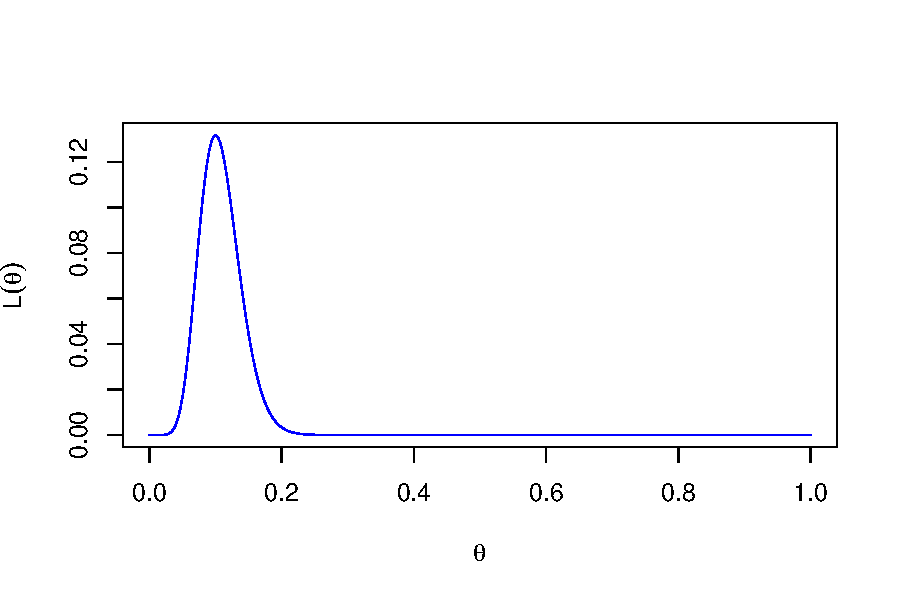
\includegraphics[width=0.55\textwidth]{thetalikelihood.pdf}
\label{fig:thetalikelihood}
\end{figure}

\item \textbf{The prior distribution}: Because $\theta$ is considered to be a random variable, we need to specify a distribution for it (this is called the ``prior'' distribution). After referring to Table~\ref{tab:distributions} again, and noting that $\theta$ is a probability, we decide to use a beta distribution for this. We choose its parameters $\alpha=3$ and $\beta=6$ to reflect our prior belief in what $\theta$ is, as shown in Figure~\ref{fig:thetaprior} (with $\theta=0.3$ being most likely and $\theta$ quite unlikely to be more than 0.6).

\begin{figure}[ht!]
\caption{\small Our prior distribution for $\theta$.}
\centering
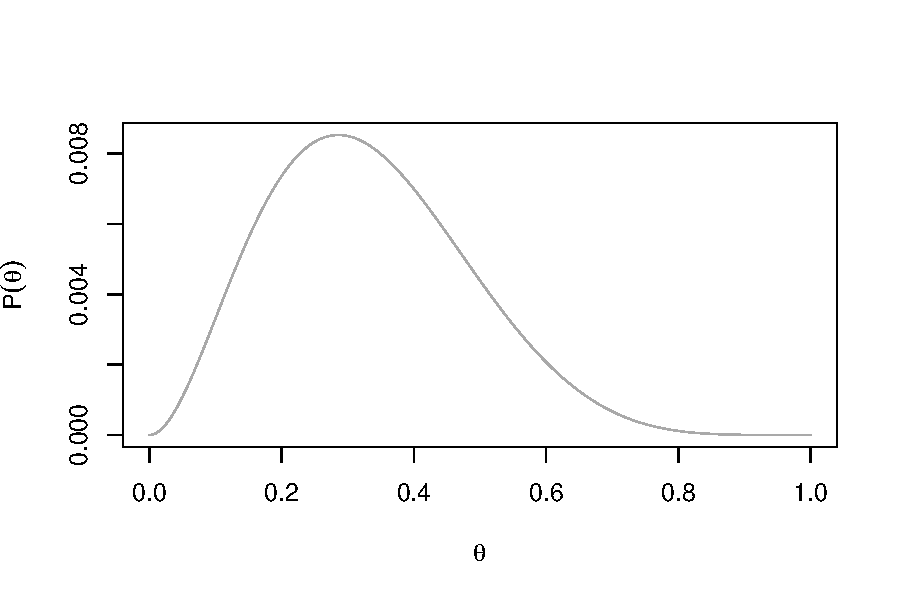
\includegraphics[width=0.55\textwidth]{thetaprior.pdf}
\label{fig:thetaprior}
\end{figure}

\item \textbf{The posterior distribution}: Armed with our likelihood $L(\theta)=P(y;\theta)$ and our prior distribution $P(\theta)$ for $\theta$, we use Bayes' Theorem to obtain the \textbf{posterior} distribution for $\theta$:

\be
P(A|B)&=&\frac{P(B|A)P(A)}{P(B)}\;=\;\frac{P(B|A)P(A)}{\int P(B|A)P(A)\;dA} \nonumber \\
P(\theta | y=10)&=&\frac{P(y=10|\theta)P(\theta)}{\int_0^1 P(y=10|\theta)P(\theta)\;d\theta}
\ee

Figure~\ref{fig:thetaposterior} shows the posterior distribution $P(\theta | y=10)$, overlaid on the prior and likelihood (scaled to integrate to 1 for comparability with the prior and posterior). You can see that the posterior distribution has been pulled a bit towards the prior (i.e. to the right), but not much and has a much narrower distribution than the prior. This indicates that the data contains a lot of information about $\theta$. If the data contained little information, the posterior would look more like the proir (the data will not have changed your prior belief much).

\begin{figure}[ht!]
\caption{\small The prior (grey dashed line), likelihood (blue dashed line) and posterior distribution (black line) of $\theta$.}
\centering
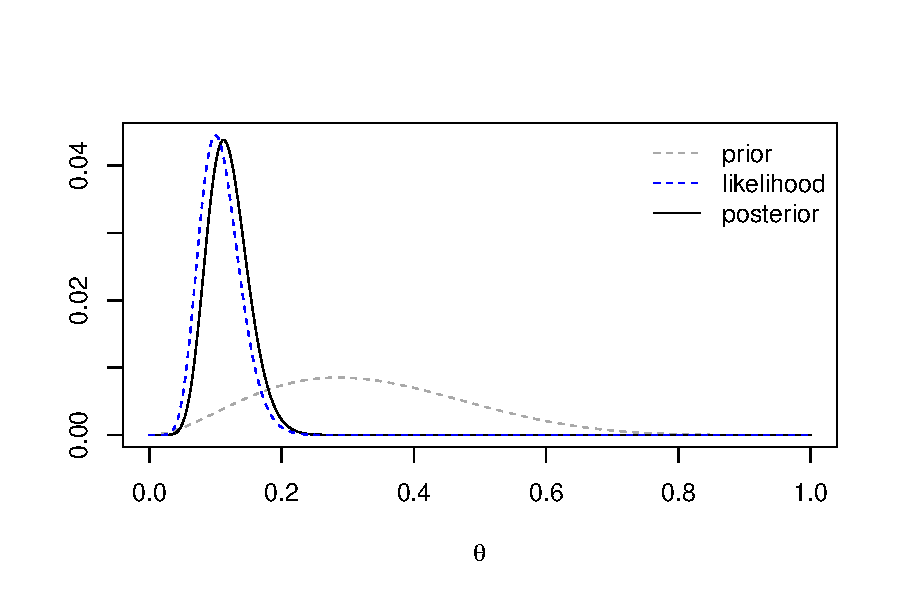
\includegraphics[width=0.7\textwidth]{thetaposterior.pdf}
\label{fig:thetaposterior}
\end{figure}
\nonumber

The posterior distribution (the black line in Figure~\ref{fig:thetaposterior}) is the Bayesian estimator for $\theta$. Notice that it is a distribution, not a single number. This is one of the attractive features of Bayesian estimators - they summarise in a probability distribution all that we know about the thing we are estimating, incuding the uncertainty and the most likely values. 

\een

In a similar way to the way that we get confidence intervals for parameters from the sampling distribution of a frequentist estimator, we get the Bayesian equivalent, ``credible intervals'' from the posterior distribution when doing Bayesian inference.

As a rule, if you use what is called an ``uninformative prior'' distribution (i.e. a prior distribution that equates to ``I have no prior knowledge of what $\theta$ is.''), then the value of $\theta$ at which the maximum of the Bayesian posterior distribution occurs, is the MLE of the parameter. (In our example, an uninformative prior would be one that assigns equal probability density to every value of $\theta$ between 0 and 1.)

Thought about in another way, the knowledge about $\theta$ that you encapsulate in the prior distribution, moves the most likely value for $\theta$ away from what it would be if you knew nothing about $\theta$ and only used the data $y_1,\ldots,n$ to inform you about it. And the MLE corresponds to the case in which you know nothing about $\theta$ before you take your sample.

\subsection{Bayesian Inference - an ecological perspective}

The above has shown how Bayesian inference works for a particular example, but the same ideas and methods apply whatever inference problem you are addressing. There are a growing number of ecological statisitcs texts that offer explanations of Bayesian inference from an ecological perspective. These resources are extrememly useful for reinforcing general statistical concepts by linking them to concrete and familiar ecological inference problems. 
The following two review papers describe why Bayesian inference should be of general interest to ecologists:

\begin{itemize}
\item Aaron, E. M. 2004. Bayesian inference in ecology. Ecology Letters 7:509–520. (\href{https://tinyurl.com/ya7d57qk}{PDF})
\item Clark, J. S. 2005. Why environmental scientists are becoming Bayesians. 8: 2-14 (\href{https://tinyurl.com/ycguf6w9}{PDF})
\end{itemize}

The following books are ``Bayesian statistics for ecologists`` reference books and the identified chapters are the ``Bayesian primer`` chapters:

\begin{itemize}
\item Kéry, M., 2010. Introduction to WinBUGS for ecologists: Bayesian approach to regression, ANOVA, mixed models and related analyses. Academic Press. Chapter 2 (\href{https://tinyurl.com/ycguf6w9}{PDF})
\item Kéry, M. and Schaub, M., 2011. Bayesian population analysis using WinBUGS: a hierarchical perspective. Academic Press. Chapter 2 (\href{https://tinyurl.com/ydyl9ont}{PDF})
\end{itemize}
